\documentclass[conference]{IEEEtran}
\IEEEoverridecommandlockouts
% The preceding line is only needed to identify funding in the first footnote. If that is unneeded, please comment it out.
\usepackage{cite}
\usepackage{amsmath,amssymb,amsfonts}
\usepackage{algorithmic}
\usepackage{graphicx}
\usepackage{textcomp}
\usepackage{enumitem}
\usepackage{xcolor}
\usepackage{booktabs}
\usepackage{fancyhdr}
\fancypagestyle{mycustomstyle}{
  \fancyhf{}  % clear header and footer
  \fancyfoot[C]{Movie Revenue Prediction}
  \fancyfoot[R]{\thepage}  % page number on the right side
}
\pagestyle{mycustomstyle}
\renewcommand{\headrulewidth}{0pt} % remove header line
\usepackage{colortbl}
\definecolor{Green}{rgb}{0.0, 1, 0.0}
\definecolor{Red}{rgb}{1.2, 0.0, 0.0}
\def\BibTeX{{\rm B\kern-.05em{\sc i\kern-.025em b}\kern-.08em
    T\kern-.1667em\lower.7ex\hbox{E}\kern-.125emX}}
\begin{document}

\title{Movie Revenue Prediction\\
{\footnotesize CIS530 Advanced Data Mining Project Report}
\thanks{}
}

\author{\IEEEauthorblockN{Phani Abhiram Raju Adidam Mohan Sai Venkata}
\IEEEauthorblockA{\textit{Graduate Student} \\
\textit{College of Engineering}\\
\textit{Data Science Program}\\
\textit{University of Massachusetts, Dartmouth}\\
ID - 02073172 \\
aphaniabhiramraju@umassd.edu}
\and
\IEEEauthorblockN{Jeevan Ravi Kumar}
\IEEEauthorblockA{\textit{Graduate Student} \\
\textit{College of Engineering}\\
\textit{Data Science Program}\\
\textit{University of Massachusetts, Dartmouth}\\
ID - 02009594 \\
jravikumar@umassd.edu}
}

\maketitle

\begin{abstract}
The film industry, characterized by its dynamic nature and fierce competition, demands strategic foresight to successfully navigate the complexities of movie production. Accurately predicting a movie's revenue before its release is a formidable and crucial challenge. Such predictions empower stakeholders to make well-informed decisions about marketing strategies, distribution plans, and other critical aspects, ultimately shaping a film's financial success. This project sets out on a pioneering journey, delving deep into the multifaceted features that may significantly impact a movie's revenue. The overarching goal is to develop a robust predictive model capable of estimating a movie's revenue with precision.\\
\end{abstract}

\textbf{\textit{Keywords}} - Movies, IMDB, Revenue, Linear Regression, Decision Trees, Random Forests, Accuracy, RMSE, R\textsuperscript{2} score.

\section{Introduction}
In film production's fast-paced and competitive realm, where uncertainty looms large, the ability to foresee a movie's financial success has become paramount. The Movie Revenue Prediction project emerges as a response to this imperative need, seeking to unravel the intricate web of factors influencing a film's revenue. By leveraging advanced data analytics and machine learning techniques, this project aims to create a predictive model that goes beyond traditional methods, incorporating diverse features to enhance accuracy.\\
The analysis will encompass an exhaustive examination of critical features such as budget, genre, production companies, countries of release, release dates, and runtime. These features, individually and collectively, play pivotal roles in determining a movie's performance at the box office. The study will delve into historical data, drawing insights from a vast array of movies spanning different genres, budgets, and production contexts. This extensive dataset will serve as the foundation for training and validating the predictive model.\\

The project's significance lies in its potential to revolutionize decision-making processes within the film industry. The model's predictive insights benefit stakeholders, including producers, distributors, and marketers. Such foresight enables them to optimize budget allocations, effectively tailor marketing campaigns to target audiences, and strategically plan release schedules for maximum impact.\\
\subsection{Business Objective and Constraints}
\begin{enumerate}
    \item \textit{Objective:}\\
    The primary business objective of the Movie Revenue Prediction project is to develop a robust and accurate predictive model that estimates the revenue of movies before their release. This predictive tool aims to provide stakeholders in the film industry with actionable insights to make informed decisions regarding marketing strategies, distribution plans, and resource allocations. By leveraging advanced data analytics and machine learning techniques, the project seeks to enhance the efficiency and effectiveness of decision-making processes within the industry.\\
    \item \textit{Constraints:}
    \begin{itemize}
        \item \textit{Data Quality and Availability}: The success of the predictive model heavily relies on the quality and availability of historical data. Inaccurate or incomplete data can compromise the model's accuracy and reliability.

        \item \textit{Budget Limitations}: While predicting revenue is essential, the project operates within the constraints of budget limitations. Striking a balance between the depth of analysis and available resources is crucial.

        \item \textit{Dynamic Industry Landscape}: The film industry is dynamic and constantly evolving, with trends changing rapidly. The predictive model must adapt to evolving market dynamics and trends to remain relevant.

        \item \textit{Privacy and Confidentiality}: Handling data related to movie budgets, revenues, and other sensitive information requires strict adherence to privacy and confidentiality standards. Compliance with legal and ethical considerations is paramount.

        \item \textit{Model Interpretability}: For stakeholders to trust and use the predictive model, it is essential that the model's predictions are interpretable. Ensuring transparency in how the model arrives at its predictions is critical.

        \item \textit{Generalization Across Genres and Regions}: The model should aim for a degree of generalization across different movie genres and regions. However, it's important to acknowledge that certain genres or regions may have unique characteristics that require specific considerations.

        \item \textit{Marketing and External Factors}: The success of a movie is influenced by various external factors, including market competition, economic conditions, and unforeseen events. The model should recognize these external influences and provide insights within this context.

        \item \textit{User-Friendliness}: The predictive model should be designed with user-friendliness in mind, ensuring that stakeholders with varying levels of technical expertise can easily interpret and utilize the generated predictions.
    \end{itemize}
\end{enumerate}

\section{Materials and Methods}

\subsection{Dataset}

The TMDB 5000 dataset refers to a movie dataset available on TMDb (The Movie Database), an online database for movies, TV shows, and celebrities. This dataset provides information on a diverse collection of movies and is often used for educational and research purposes in the field of data science and machine learning.\\
The TMDB 5000 dataset typically includes a range of features for each movie, offering insights into various aspects of the film industry. Some common attributes found in such datasets may include:
\begin{itemize}
    \item \textbf{Movie ID}: A unique identifier for each movie.
    \item \textbf{Title}: The title of the movie.
    \item \textbf{Budget}: The budget allocated for producing the movie.
    \item \textbf{Revenue}: The revenue generated by the movie. 
    \item \textbf{Genres}: The genre(s) to which the movie belongs.
    \item \textbf{Release Date}: The date when the movie was released.
    \item \textbf{Runtime}: The duration of the movie in minutes.
    \item \textbf{Popularity}: A measure of the movie's popularity on TMDb.
    \item \textbf{Vote Average}: The average rating users give the movie.
    \item \textbf{Vote Count}: The number of user votes received.
    \item \textbf{Production Countries}: The countries where the movies was produced in.
    \item \textbf{Cast}: The list of cast starring in each movie.
    \item \textbf{Crew}: The list of crew who worked on the movie.
\end{itemize}

\subsection{Exploratory Data Analysis}
\begin{itemize}
    \item Several insights can be derived based on the exploratory data analysis (EDA) conducted on the TMDB 5000 dataset. The scatter plot and regression plot depicting the relationship between budget and revenue reveal a positive correlation, suggesting that higher budgets are associated with higher revenue, which is in line with industry expectations.\\
    \item Additionally, the line chart illustrating the number of movies released over time indicates a gradual increase in movie production, reflecting the growth or evolution of the film industry. However, a more comprehensive analysis, including a deeper examination of specific periods, might provide a nuanced understanding of the temporal trends.\\
    \item The word cloud generated from movie overviews offers insights into the prevalent themes or topics within the dataset. Frequently occurring words, such as 'love,' 'power,' 'family,' or genre-related terms, can give a sense of the common narrative elements present in these movies. This information can be valuable for content creators, marketers, and analysts in understanding the thematic landscape of the films included in the dataset.\\
    \item  Overall, the combination of scatter plots, line charts, regression plots, and word clouds provides a multifaceted perspective on the TMDB 5000 dataset, offering insights into both quantitative relationships and qualitative aspects of the movies it encompasses. Below are the plots and graphs generated:\\
\end{itemize}
 
\begin{figure}[htbp]
    \centerline{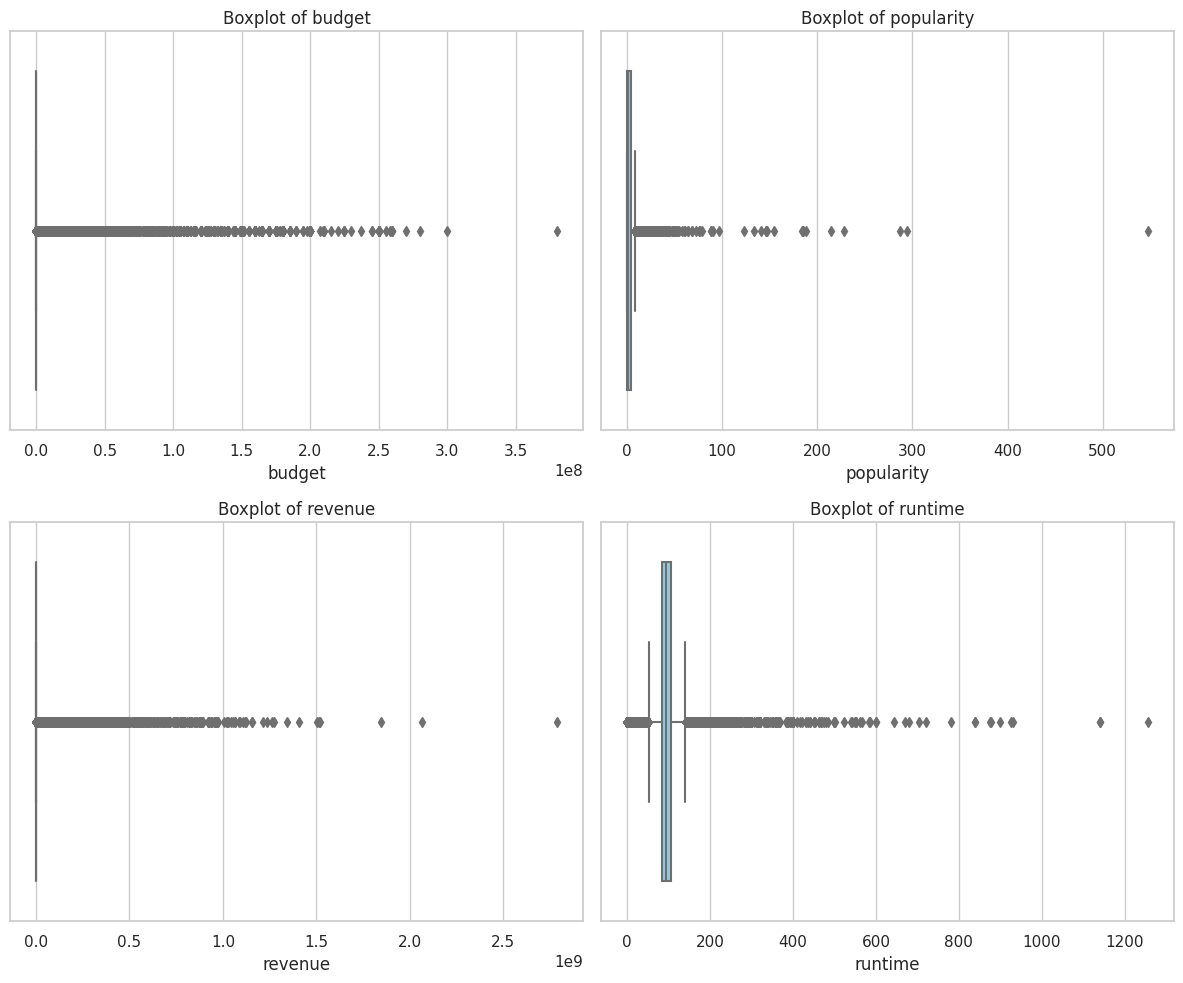
\includegraphics[width=0.45\textwidth]{boxplots_budget_runtime_revenue_popularity.png}}
    \caption{Boxplots of Budget, Runtime, Revenue and Popularity}
    \label{fig:enter-label}
\end{figure}

\begin{figure}[htbp]
    \centerline{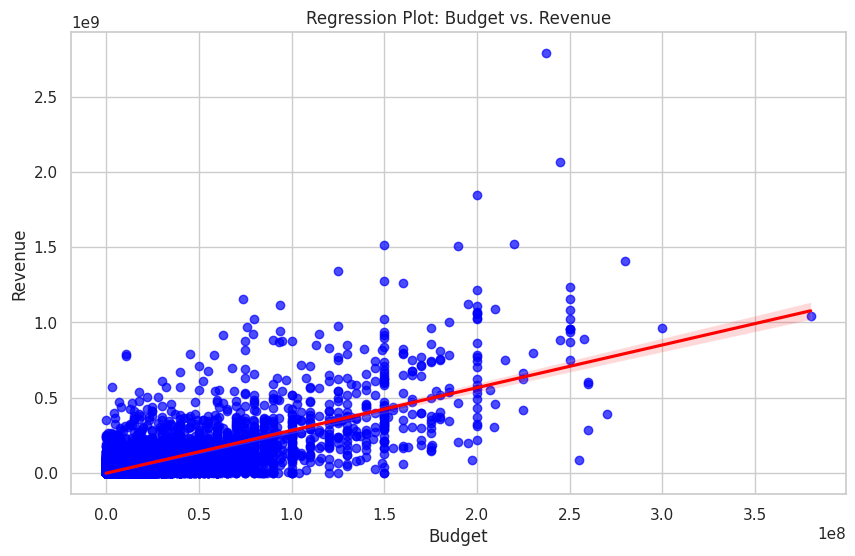
\includegraphics[width=0.45\textwidth]{budget_vs_rev_regplot.png}}
    \caption{Regresssion plot of Budget VS Revenue}
    \label{fig:enter-label}
\end{figure}

\begin{figure}[htbp]
    \centerline{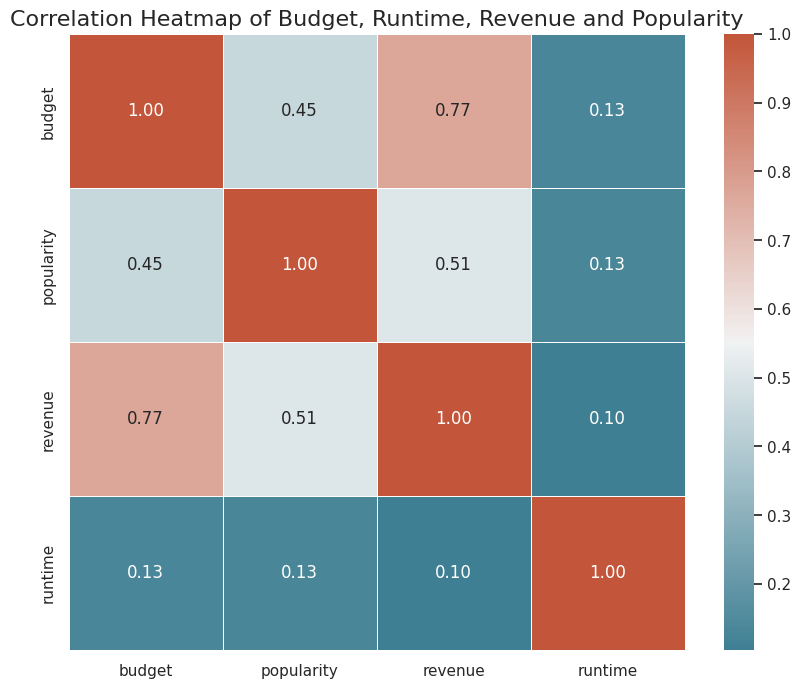
\includegraphics[width=0.45\textwidth]{corrplot_budget_runtime_revenue_popularity.png}}
    \caption{Heatmap correlation of Budget, Runtime, Rvenue and Popularity}
    \label{fig:enter-label}
\end{figure}    

\begin{figure}[htbp]
    \centerline{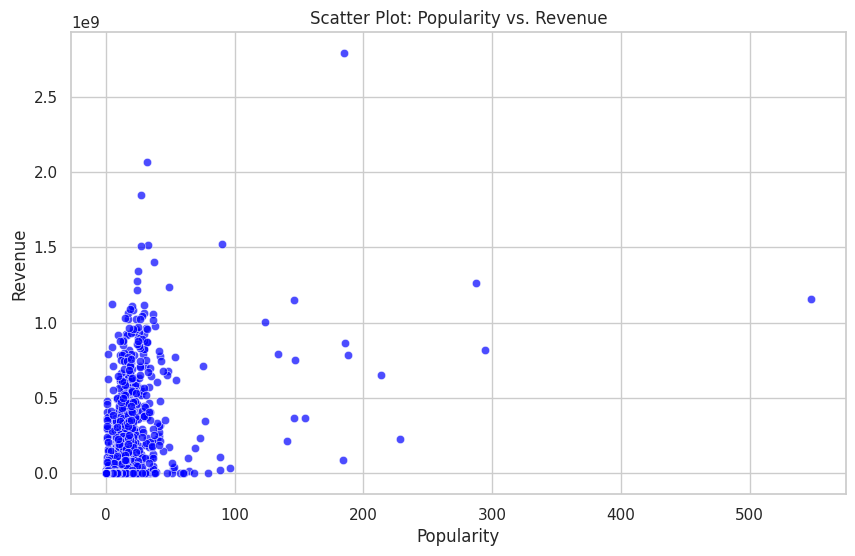
\includegraphics[width=0.45\textwidth]{pop_vs_rev_scatter.png}}
    \caption{Scatter plot distribution between Popularity and Revenue}
    \label{fig:enter-label}
\end{figure}   

\begin{figure}[htbp]
    \centerline{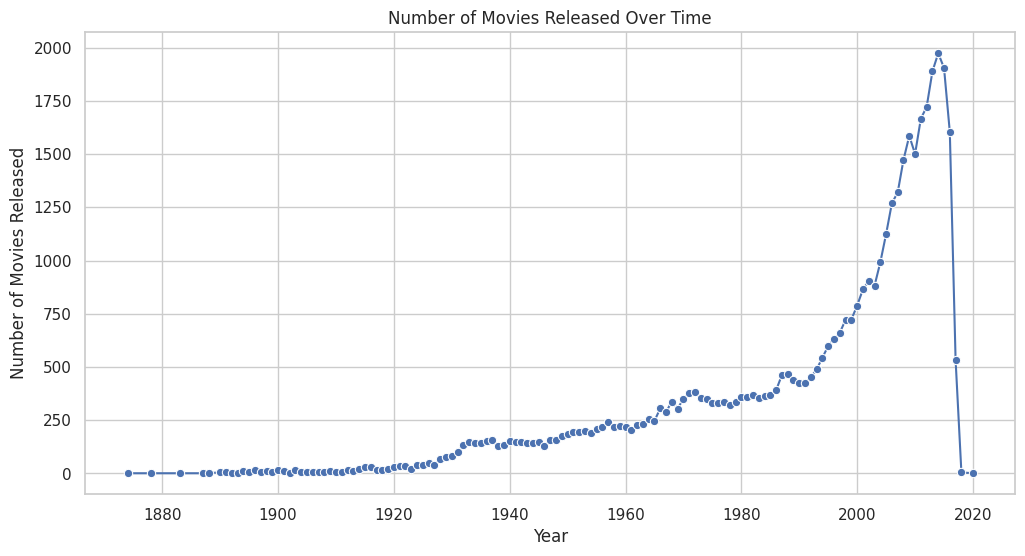
\includegraphics[width=0.45\textwidth]{release_date_trend.png}}
    \caption{Trend of Movies released every year}
    \label{fig:enter-label}
\end{figure}   

\begin{figure}[htbp]
    \centerline{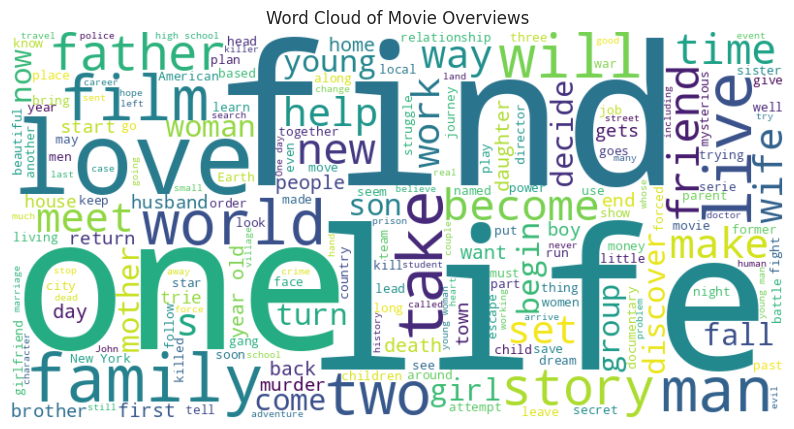
\includegraphics[width=0.45\textwidth]{wordcloud_overview.png}}
    \caption{Worldcloud of Movie plots}
    \label{fig:enter-label}
\end{figure}   

\newpage
\subsection{Data Transformations}

\begin{itemize}
    \item \textbf{\textit{Column Removal}}: Identified and dropped irrelevant columns such as tagline, belongs-to-collection, homepage, poster-path, status, video, and original-title as they were deemed non-contributory to revenue prediction.
    \item \textbf{\textit{Handling Duplicates}}: Detected and removed 987 duplicates from the keywords dataset to ensure the integrity of the data.
    \item \textbf{\textit{Dataset Merge}}: Merged the primary dataset with the cleaned keywords dataset using the 'id' column, consolidating relevant information.
    \item \textbf{\textit{Numeric Conversion}}: Ensured 'revenue' and 'budget' columns were of numeric type, converting them if necessary to facilitate model training.
    \item \textbf{\textit{Zero-Value Rows Removal}}: Eliminated rows where both 'revenue' and 'budget' were zero, preventing potential distortions in the model.
    \item \textbf{\textit{Missing Value Imputation}}: Imputed mode values for missing entries in the 'revenue' and 'budget' columns to maintain dataset completeness.
    \item \textbf{\textit{Data Extraction Using literal-eval function}}: Utilized the literal-eval function to extract structured information from the 'genre', 'production-companies','production-countries,' 'spoken-languages,' and 'keywords' columns.
    \item \textbf{\textit{Crew Information Extraction}}: Extracted director names from the crew list to facilitate analysis of directorial impact on revenue.
    \item \textbf{\textit{Lead Actor Extraction}}: Extracted lead actor names from the cast list to capture their potential influence on revenue.
    \item \textbf{\textit{Date Information Extraction}}: Created new columns, 'release-month' and 'release-day,' derived from the 'release-date' column for temporal analysis.
    \item \textbf{\textit{Language Standardization}}: Mapped the top 10 most frequently used languages, replacing language codes with their corresponding names for consistency.
    \item \textbf{\textit{Genre Simplification}}: Extracted the first three genres from each movie, simplifying genre information for analysis.
    \item \textbf{\textit{Categorical Mapping}}: Developed mapping dictionaries for 'genres' and 'original-language,' converting them into numerical values to facilitate model input.
    \item \textbf{\textit{Additional Numeric Conversion}}: Ensured the 'revenue' and 'budget' columns were consistently numeric.
    \item \textbf{\textit{Director and Lead Actor Mapping}}: Created numerical mappings for 'director' and 'lead-actor' for model compatibility.
    \item \textbf{\textit{Country Standardization}}: Identified and replaced the top 10 countries by percentage with their corresponding numerical mappings.
    \item \textbf{\textit{Winsorization}}: Applied Winsorization to 'revenue' and 'budget' columns at the 1st and 99th percentiles to mitigate the impact of outliers.
    \item \textbf{\textit{Sentiment Analysis}}: Implemented sentiment analysis using the TextBlob function on the 'overview' and 'keywords' columns, replacing them with equivalent sentiment scores for enriched features.
\end{itemize}

\section{Model - Training and Testing}

\subsection{Models and Libraries chosen}
The code utilizes scikit-learn, a powerful machine learning library in Python, to implement and compare two regression models: Linear Regression and Random Forest Regressor. These models are selected for their suitability in predicting numeric values, particularly in the context of revenue prediction.

\subsection{Separating Features and Target Variables}
The DataFrame' data' represents the dataset,' and is organized with features and a target variable ('revenue'). The code efficiently employs scikit-learn to segregate the features (X) from the target variable (y). This step ensures that the models are trained on independent variables to predict the dependent variable.

\subsection{Splitting the Dataset into Training and Testing}
The code employs the train-test-split function from scikit-learn to partition the dataset into distinct training and testing sets. The training set (X-train, y-train) is utilized for model training, while the reserved testing set (X-test, y-test) is employed for robust model evaluation. A test size of 20 percent and a consistent random state (42) are specified to maintain reproducibility.

\subsection{Feature Scaling}
Standardization, facilitated by scikit-learn's StandardScaler, is applied to ensure uniform scaling across all features. This essential preprocessing step prevents any particular feature from dominating the model due to disparate magnitudes, promoting stability and convergence.

\subsection{Applying the Linear Regression Model}
The code initializes a Linear Regression model, trains it on the scaled training data, and subsequently predicts the target variable on the scaled testing data. Evaluation metrics, including Root Mean Squared Error (RMSE) and R-squared (R\textsuperscript{2}) score, are computed to gauge the performance of the Linear Regression model.

\subsection{Applying the Random Forest Model}
Similarly, a Random Forest Regressor model is initiated, trained on the scaled training data, and leveraged for predictions on the testing set. Evaluation metrics, RMSE and R\textsuperscript{2} score, are then computed to assess the Random Forest model's performance.

\subsection{Comparing the Models Performances}
The code generates a dictionary, 'model-performance,' encapsulating the computed evaluation metrics for both the Linear Regression and Random Forest models. This includes RMSE, a measure of prediction error, and R\textsuperscript{2} score, indicating the proportion of variance explained by the models. The presented performance metrics provide a clear and concise basis for direct model comparison.

\begin{table}[htbp]
    \centering
    \caption{Model Performance}
    \begin{tabular}{lcc}
    \toprule
    \textbf{Model} & \textbf{RMSE} & \textbf{R\textsuperscript{2} score} \\
    \midrule
    Linear Regression & 56,659,160.06 & 0.75 \\
    Random Forest & 49,663,714.65 & 0.81 \\
    \bottomrule
    \end{tabular}
\end{table}

\section{Pickling the selected model}

In the process of model selection, the emphasis often lies on identifying the model that exhibits the highest R\textsuperscript{2} score, indicative of superior predictive performance. In the given scenario, a Random Forest Regressor model ('rf-model') has demonstrated promising R\textsuperscript{2} scores during training and testing. To streamline this selected model's deployment and future usage, the code employs the joblib module in conjunction with scikit-learn's Pipeline function. This combination encapsulates the entire modeling process, including the scaling of features using the 'scaler' and the application of the Random Forest model. The Pipeline ensures a seamless integration of preprocessing steps with the model, maintaining consistency in data transformations during both training and inference. Subsequently, the joblib.dump function is employed to serialize the entire pipeline, storing it in a file named 'random-forest-model.pkl'. This pickled file becomes a portable representation of the complete modeling workflow, facilitating easy and efficient deployment for future predictions without the need to retrain the model.

\section{Deploying an Integrated Web Application}

The Python code file 'main.py' establishes a FastAPI web application for movie revenue prediction. It utilizes a pre-trained Random Forest https://www.overleaf.com/project/657bbc90f21270f6ba4a773amodel, loaded through the joblib module, and incorporates scikit-learn's Pipeline functionality for seamless integration of preprocessing steps. The model takes various movie-related inputs, such as budget, language, overview, popularity, runtime, and more, submitted through an HTML form. The form is designed with fields for the user to input relevant information, including checkboxes, number inputs, text areas, and dropdowns for genres, directors, and lead actors.\\

Upon submitting the form, the entered data is processed on the server side, applying sentiment analysis to the 'overview' and 'keywords' columns, dropping unnecessary columns, and predicting the movie's revenue using the pre-trained Random Forest model. The predicted revenue is then returned as a response.\\

The accompanying HTML and JavaScript code defines the structure and interactivity of the web application. It sets up a visually appealing user interface with input fields, checkboxes, and buttons. JavaScript handles form submission, triggering an asynchronous fetch request to the '/process' endpoint of the FastAPI application. The predicted revenue is dynamically displayed on the webpage, along with a verdict on the movie's potential profitability based on a comparison with the entered budget.\\

This end-to-end integration showcases the utilization of machine learning models, preprocessing techniques, and a web framework to create an interactive tool for predicting movie revenues. Users can input various features, receive revenue predictions, and obtain insights into the potential financial success of their hypothetical movies.\\

\begin{figure}[htbp]
    \centerline{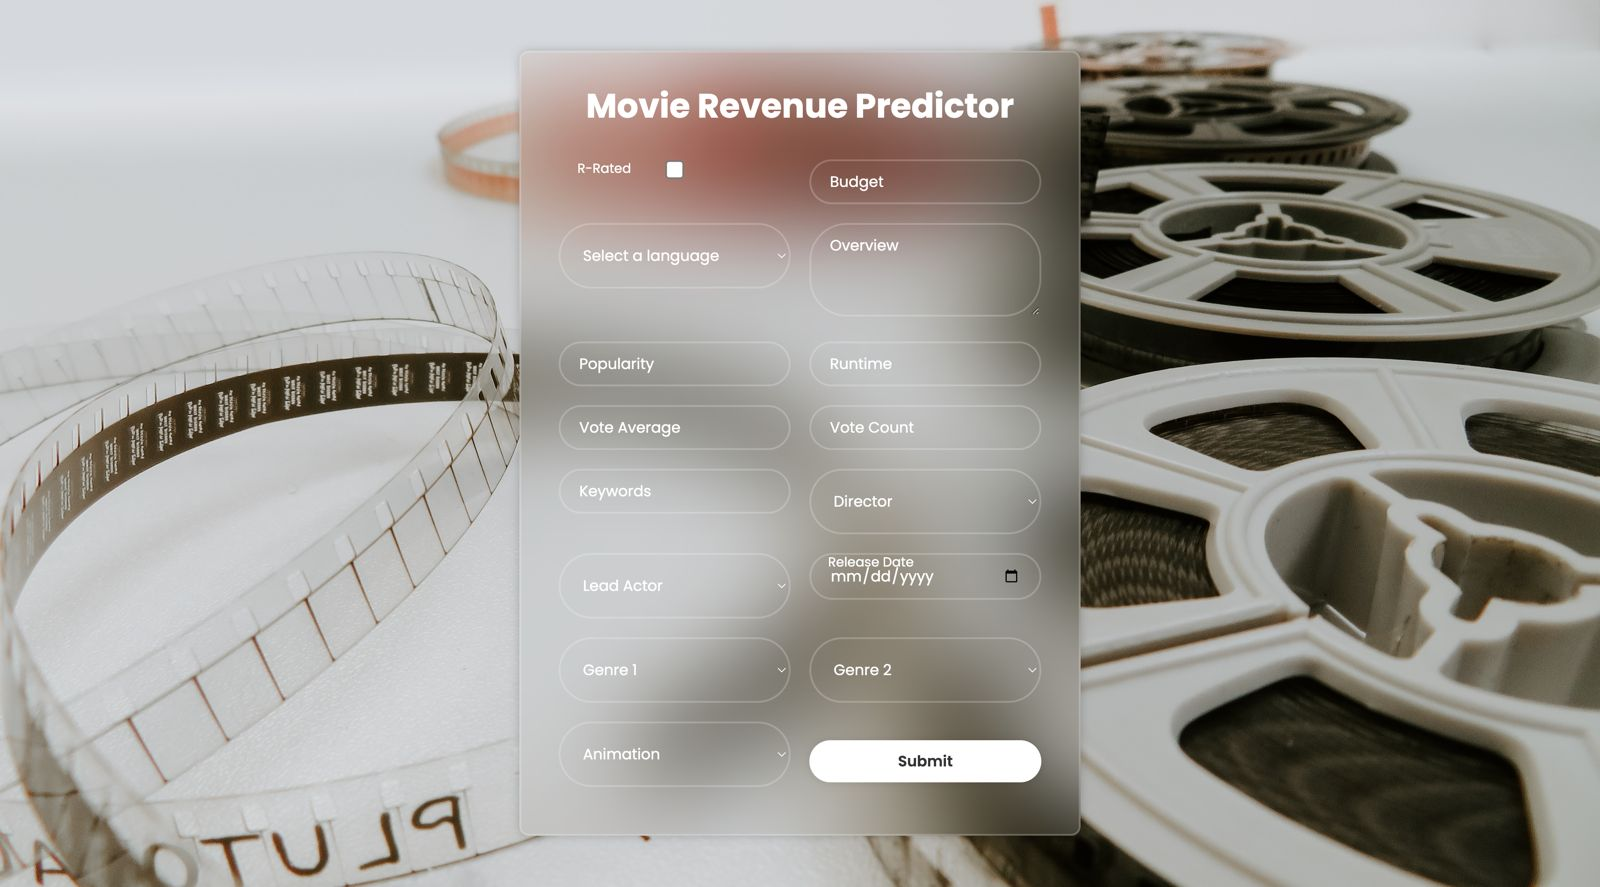
\includegraphics[width=0.45\textwidth]{webpage_sc.jpg}}
    \caption{The webpage}
    \label{fig:enter-label}
\end{figure}

\section{Conclusion}

In this project, we thoroughly explored the TMDB 5000 dataset, employing exploratory data analysis and visualization techniques to understand trends and patterns in the movie industry. Subsequent data preprocessing involved handling missing values, transforming variables, and applying sentiment analysis. We trained Linear Regression and Random Forest models for revenue prediction, assessing their performance metrics. The deployment of a FastAPI web application showcased the practical application of the Random Forest model for real-time revenue forecasts. This end-to-end process demonstrated the versatility of machine learning in extracting insights from data and deploying predictive models in a user-friendly interface, emphasizing the interdisciplinary nature of data science.

\begin{thebibliography}{00}
\bibitem{b1} Kaggle [https://www.kaggle.com/code/victorpaschoalini/movies-eda-revenue-prediction]
\bibitem{b2} Dataset - Kaggle [https://www.kaggle.com/datasets/tmdb/tmdb-movie-metadata/data]
\bibitem{b3} MachineLearningMastery [https://machinelearningmastery.com/columntransformer-for-numerical-and-categorical-data/]
\bibitem{b4} MachineLearningMastery [https://machinelearningmastery.com/columntransformer-for-numerical-and-categorical-data/]
\bibitem{b5} Towardsdatascience [https://towardsdatascience.com/how-to-combine-textual-and-numerical-features-for-machine-learning-in-python-dc1526ca94d9]
\bibitem{b6} Medium [https://medium.com/analytics-vidhya/serve-a-machine-learning-model-using-sklearn-fastapi-and-docker-85aabf96729b]
\bibitem{b7} section.io [https://www.section.io/engineering-education/how-to-create-a-machine-learning-app-using-the-fastapi-and-deploying-it-to-the-kubernetes-cluster/]
\end{thebibliography}

\end{document}
